\documentclass[11pt, twocolumn]{report}

\usepackage{fullpage}
\usepackage{graphicx}
\usepackage{float}
\restylefloat{table}

\title{CCN Assignment 2: S0936300}

\begin{document}
\maketitle
\chapter{Part A}

\section{Question 1}
When the program reaches the upper boundary, $a$ which is 0.1 a decision is made in relation to hypothesis h+. If the lower boundary is reached which is 0, a decision is made in relation to the hypothesis h-. Figures \ref{p1_1_1}, \ref{p1_2}, \ref{p1_1_3} and \ref{p1_1_4} are example trials of the Wiener diffusion process.

\begin{figure}[H]
\centering
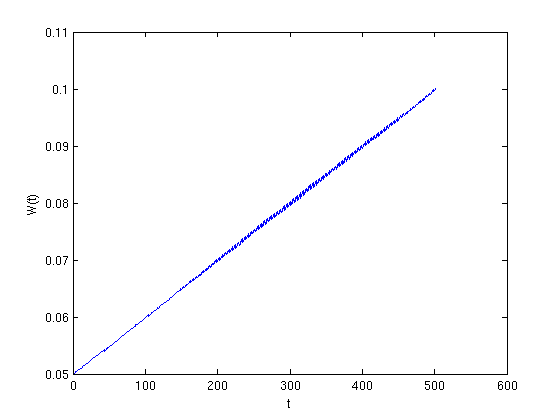
\includegraphics[width=90mm]{assignment2_images/p1_1_1.png}
\caption{Trial 1}
\label{p1_1_1}
\end{figure}

\begin{figure}[H]
\centering
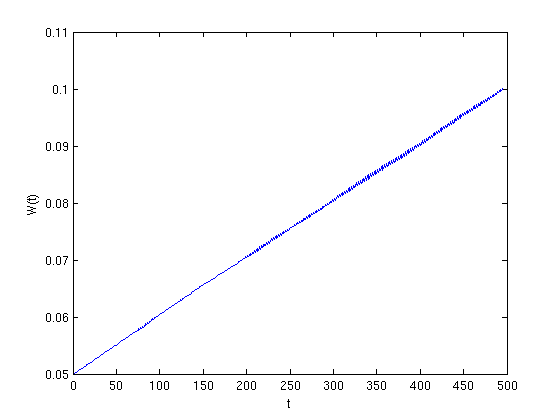
\includegraphics[width=90mm]{assignment2_images/p1_1_2.png}
\caption{Trial 2}
\label{p1_2}
\end{figure}

\begin{figure}[H]
\centering
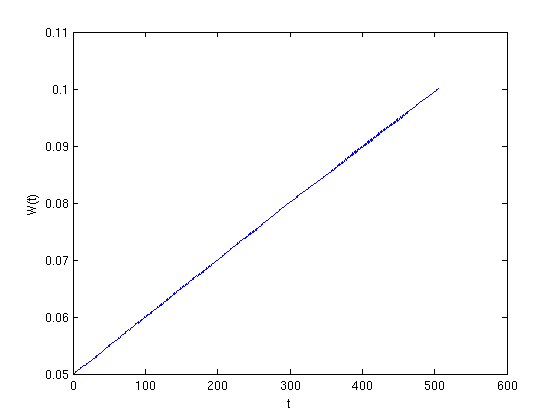
\includegraphics[width=90mm]{assignment2_images/p1_1_3.png}
\caption{Trial 3}
\label{p1_1_3}
\end{figure}

\begin{figure}[H]
\centering
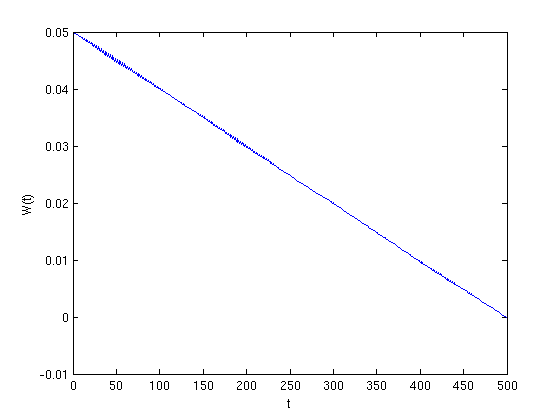
\includegraphics[width=90mm]{assignment2_images/part1_neg.png}
\caption{Trial 4: negative drift used. We can see that the opposite decision boundary is reached}
\label{p1_1_4}
\end{figure}

The program runs until either boundary is reached. In all three cases, the accumulation of information reaches the upper boundary, $a$ and thus a decision in favour of h+ is made. Inspire of errors, the reaction time(RT) is generally constant in each trial.

\section{Question 2}

By changing the drift rate $v$ we can model whether a process was easy or difficult. The prediction is that by increasing the drift rate the reaction time should reduce in addition to reducing the amount of errors; simulating an "easy" task. In contrast, by reducing the drift rate $v$, this should indicate the task is more difficult and the RT should increase as well as the amount of errors made.

\begin{figure}
\centering
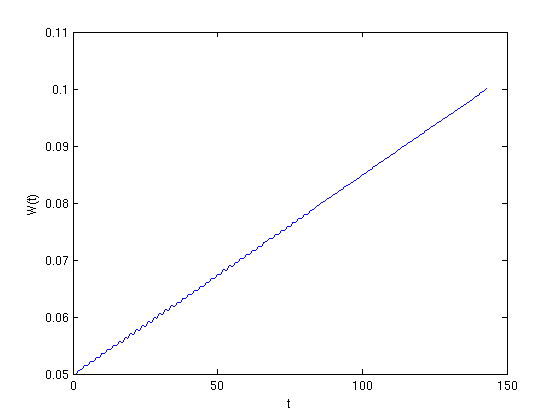
\includegraphics[width=90mm]{assignment2_images/p2/1.png}
\caption{v = 0.7}
\label{1}
\end{figure}

\begin{figure}
\centering
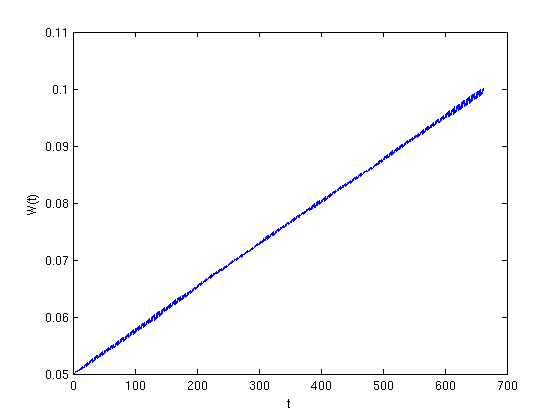
\includegraphics[width=90mm]{assignment2_images/p2/2.png}
\caption{v = 0.15}
\label{2}
\end{figure}

\begin{figure}
\centering
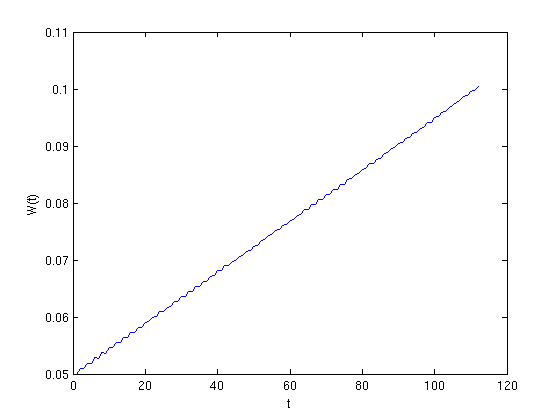
\includegraphics[width=90mm]{assignment2_images/p2/3.png}
\caption{v = 0.9}
\label{3}
\end{figure}

\begin{figure}
\centering
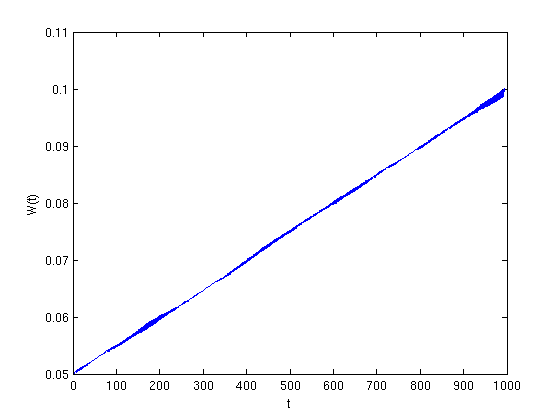
\includegraphics[width=90mm]{assignment2_images/p2/4.png}
\caption{v = 0.1}
\label{4}
\end{figure}

\begin{figure}
\centering
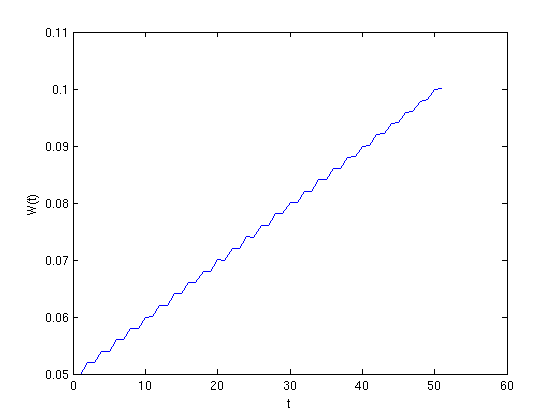
\includegraphics[width=90mm]{assignment2_images/p2/5.png}
\caption{v = 2}
\label{4}
\end{figure}


From the figures we can see that when the drift rate increases, the reaction time reduces. By increasing $v$ to 0.7(\ref{1}), the RT is reduced from 500 to approximately 150. Likewise, the reaction time increases as the drift rate decreases(see \ref{4}, \ref{2}); when the drift rate is halved to 0.1 the reaction time doubles. Errors are greater as the task is more difficult, when the drift rate is higher as in \ref{5} we can clearly see the individual errors but for the decreased drift rate there is a huge amount; it becomes troublesome to even see the individual line and it appears as one thick one. Thus the former prediction on the effects of the drift rate is experimentally seen to be correct. 

\section{Question 3}
Hypothesis: Firstly, by increasing boundaries such they are further from the start point the RT will increase. Secondly by reducing the boundaries such they are closer to the start point, the RT should reduce as speed is amplified. 

\begin{figure}[H]
\centering
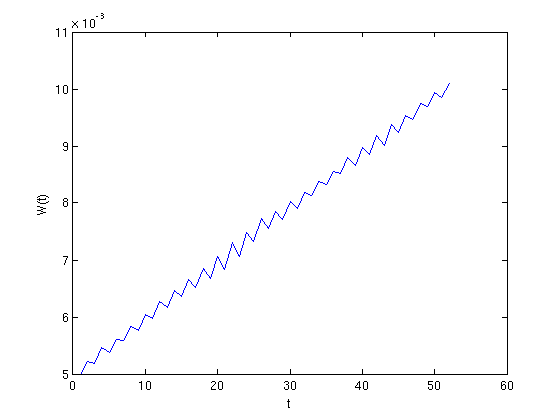
\includegraphics[width=90mm]{assignment2_images/p1_3_1a.png}
\caption{a = 0.01}
\label{p1_1_3}
\end{figure}

\begin{figure}[H]
\centering
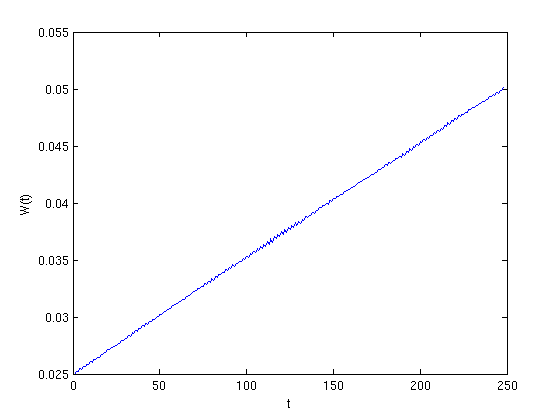
\includegraphics[width=90mm]{assignment2_images/p1_3_2a.png}
\caption{a = 0.05}
\label{p1_1_6}
\end{figure}

For both of the plots in \ref{p1_1_3} and \ref{p1_1_6}, $a$ has been reduced from 0.1 in order to make the decision boundaries closer to the starting point. We can observe that by doing this, the RT time has reduced and the former prediction is correct.

\begin{figure}[H]
\centering
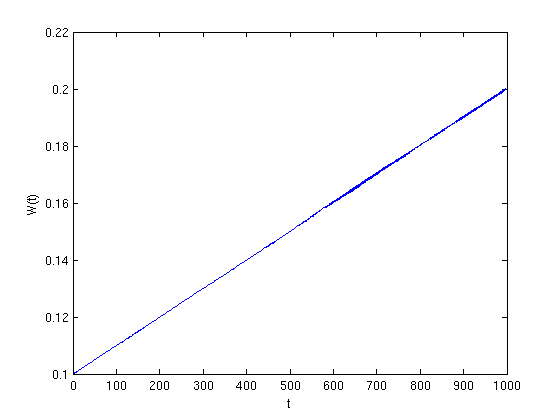
\includegraphics[width=90mm]{assignment2_images/p1_3_3a.png}
\caption{a = 0.2}
\label{p1_1_8}
\end{figure}

\begin{figure}[H]
\centering
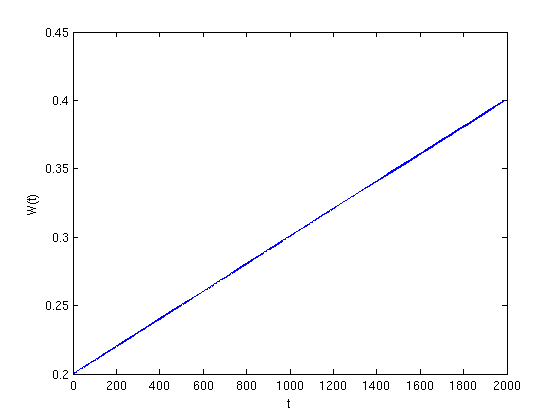
\includegraphics[width=90mm]{assignment2_images/p1_3_4a.png}
\caption{a = 0.4}
\label{p1_1_7}
\end{figure}

For both of the plots \ref{p1_1_8} and \ref{p1_1_7}, $a$ has been increased from 0.1 in order to make the decision boundaries further from the starting point. We can observe that by doing this, the RT time has increased and the former prediction is correct. 

\section{Question 4}
Variability to the drift rate was introduced in the Ratcliff diffusion process in order to more accurately model the variability of encoding in memory\cite{ratclif}. Variability in the two parameters(starting point and drift rate) can be used to account for "speed of correct verses error responses". Error responses can be quicker when a task is easier and speed is a strong factor in the decision process. 

For the drift rate when it is 400ms, the probability of a correct response is 0.95 and when the drift rate is 600ms, the probability of a correct response is 0.80. 

Varying the starting boundary does not effect obtaining the correct response but there are differences in how this is obtained. When the variability results in a starting point above the start point, accuracy is higher, RT is lower and errors are slow in contrast to when the variability in the starting point results in it becoming lower than the start point, there is lower accuracy, longer RT's and errors are fast. 

When combining variability of both parameters, error responses can be slower than correct responses but faster than correct responses at extreme levels of accuracy. 

\section{Question 5}
There are two ways I could think of. We could model prior information by changing the initial starting boundary to be closer to the boundary of one of the hypothesis. In the example given where $p(h+) = 2p(h-)$, the priors would be $\frac{2}{3}$ and $\frac{1}{3}$ for hypothesis $h+$ and $h-$ respectively. Thus the initial starting boundary to give weight to $h+$ could be moved $\frac{2}{3}$ closer to  the boundary that represents hypothesis $h+$. This would mean that if the correct decision was h+, the decision for h+ would occur more quickly, however, if it is h-, this decision will occur more slowly, but, it may not correctly change the probability such that h+ occurs 2/3 times more. The drift rate 

The log-likelihood test reveals whether one model is preferred, and thus one hypothesis is preferred over the other given the data. 

\chapter{Part B}

\section{Question 1}
Below is a table representing the values of each state after each iteration. An iteration represents moving from t=1 to t=6 and updating all the states once. 10 iterations are shown, the values of each of the states tend to 1 as expected as the last state has a reward of 1. 

\begin{figure}[H]
\centering
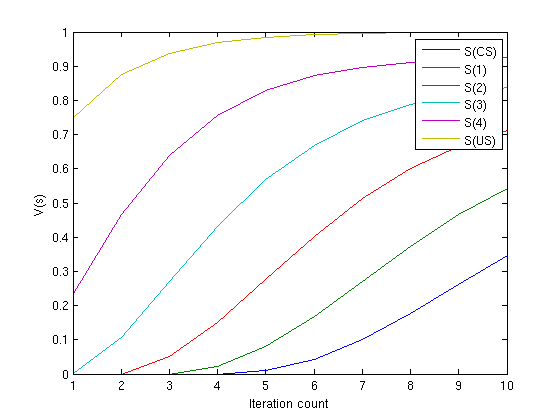
\includegraphics[width=90mm]{assignment2_images/part2_a.png}
\caption{Plot of values of each state over each iteration}
\label{values}
\end{figure}

Figure \ref{avoidance} shows the plot of avoidance probabilities over each iteration. If p(s) = 1, the agent will avoid and thus prevent themselves being shocked. As the plot shows the overall p(avoidance) converging to 1, it shows that over time they learn to avoid the stimulus. 

\begin{figure}[H]
\centering
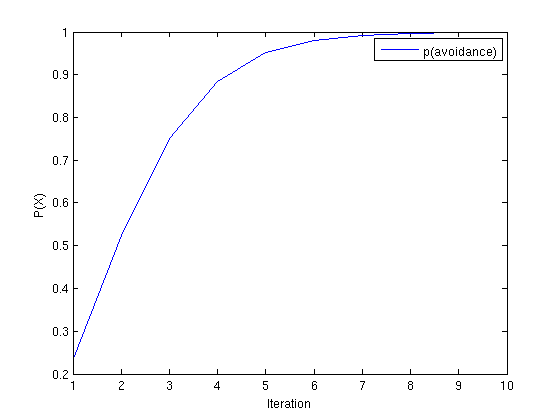
\includegraphics[width=90mm]{assignment2_images/pa.png}
\caption{Plot of P(avoidance)}
\label{avoidance}
\end{figure}

\section{Question 2}
Results from implementing dopamine:

\begin{figure}[H]
\centering
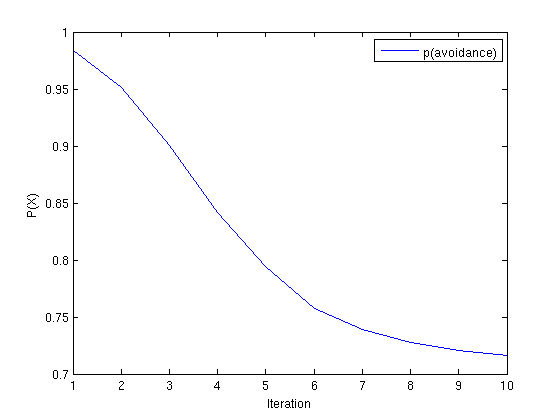
\includegraphics[width=90mm]{assignment2_images/p_av_2.png}
\caption{o = -0.2}
\label{dop1}
\end{figure}

\begin{figure}[H]
\centering
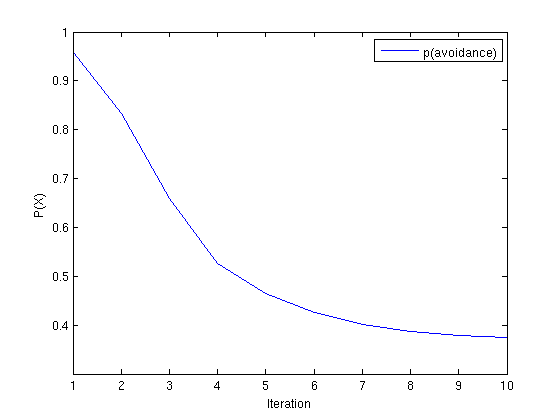
\includegraphics[width=90mm]{assignment2_images/p_av_3.png}
\caption{o = -0.3}
\label{dop2}
\end{figure}

\begin{figure}[H]
\centering
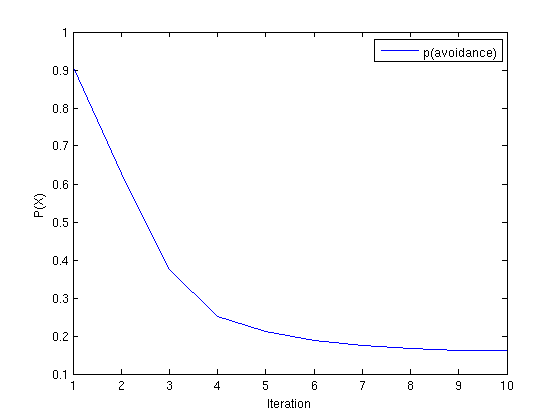
\includegraphics[width=90mm]{assignment2_images/p_av_4.png}
\caption{o = -0.4}
\label{dop3}
\end{figure}

If the value of each state was less than 0, it was set to 0. (Not sure if this is the correct way to do it, but otherwise it resulted in probabilities below zero). We observe that the avoidance probabilities decrease on each iteration and the more dopamine is blocked, the lower the probability avoidance is within the same amount of iterations. In \ref{dop1} we can see the probability of avoidance reduces to approx 0.72, however in \ref{dop3} this is even less and the probability of avoidance is -0.4. If we reduce the learning rate it can be observed that the probability is reduced.

Figures \ref{dop1}, \ref{dop2}, \ref{dop3} are all very similar, if not identical to the figures in the paper. 

\begin{thebibliography}{9}

\bibitem{ratclif} R.Ratcliff and J.N Rounder. Modeling response times for two-choice decisions. Psychological Science. 9:347-356, 1998
\end{thebibliography}

\end{document}